\section{MGADC08 - CHIME Mezzanine}
\label{sec_mezzanine}

\begin{figure}[!htbp]
	\centering
	\includegraphics[width=\linewidth]{./MezzaninePhotos/mezzcover.jpeg}
	\caption{MGADC08 mezzanine}
	\label{fig:mezz}
\end{figure}

\pagebreak
\subsection{Impedance Test}

Connect the SMA quick connect cable to one of the SMA ports on the mezzanine to provide ground - see figure \ref{fig:ImpGroundLoc}.

\begin{figure}[!htbp]
	\centering
	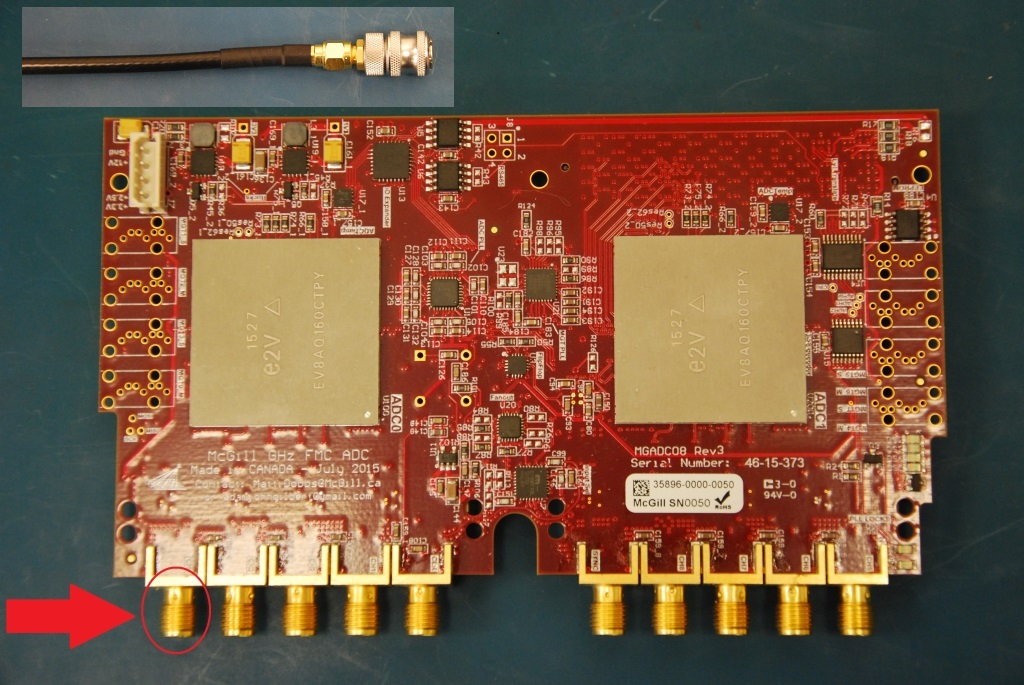
\includegraphics[height=6cm]{./MezzaninePhotos/ImpedanceTest/ImpedanceSetup.jpeg}
	\caption{Quick connect SMA ground location and quick connect SMA}	\label{fig:ImpGroundLoc}
\end{figure}

Use the red probe shown in figure \ref{fig:RedProbe} to measure impedances at the test points identified in table \ref{tab:SmokeTestPoints} below.

\begin{figure}[!htbp]
	\centering
	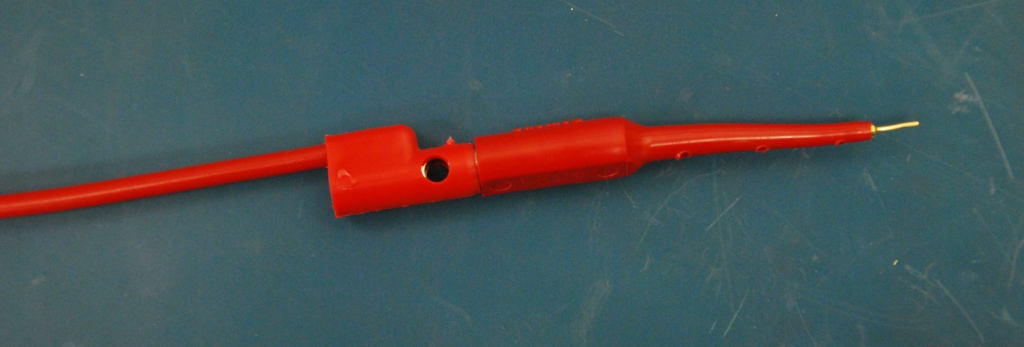
\includegraphics[height=2.5cm]{./MezzaninePhotos/ImpedanceTest/Red_Probe.jpeg}
	\caption{Red Probe}
	\label{fig:RedProbe}
\end{figure}


\begin{table}[!htbp]
	\begin{tabular}{cc}
		\begin{subfigure}{0.5\textwidth}
			\centering
			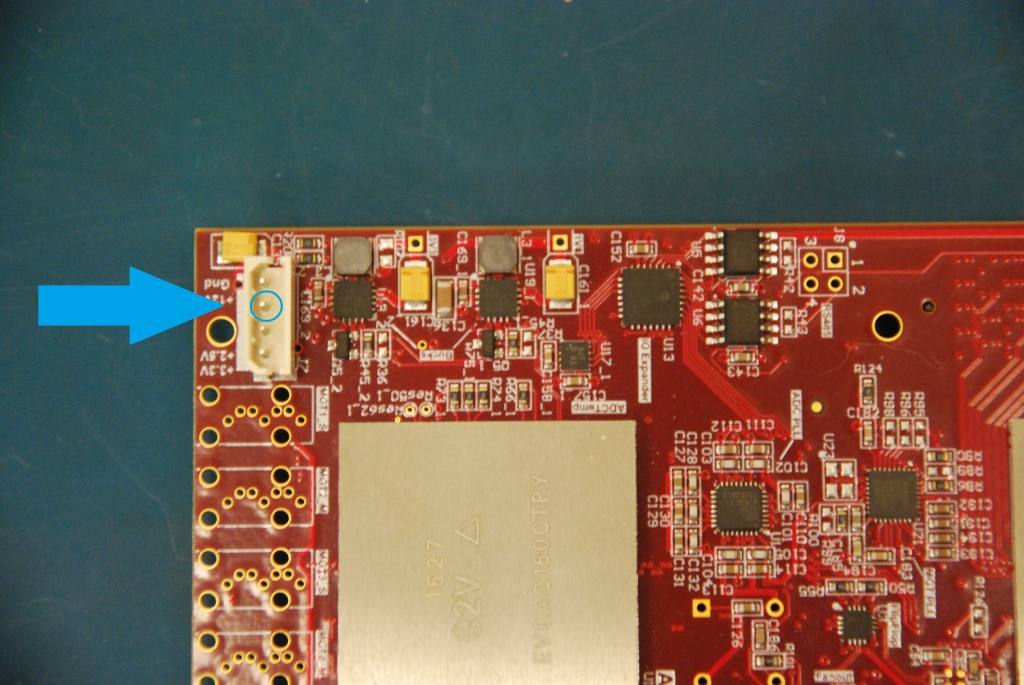
\includegraphics[width=\columnwidth]{./MezzaninePhotos/ImpedanceTest/Impedance_12V.jpeg}
			\caption{12V Probe Spot - J7 Pin2}
			\label{fig:12VProbe}
		\end{subfigure}
		&
		\begin{subfigure}{0.5\textwidth}
			\centering
			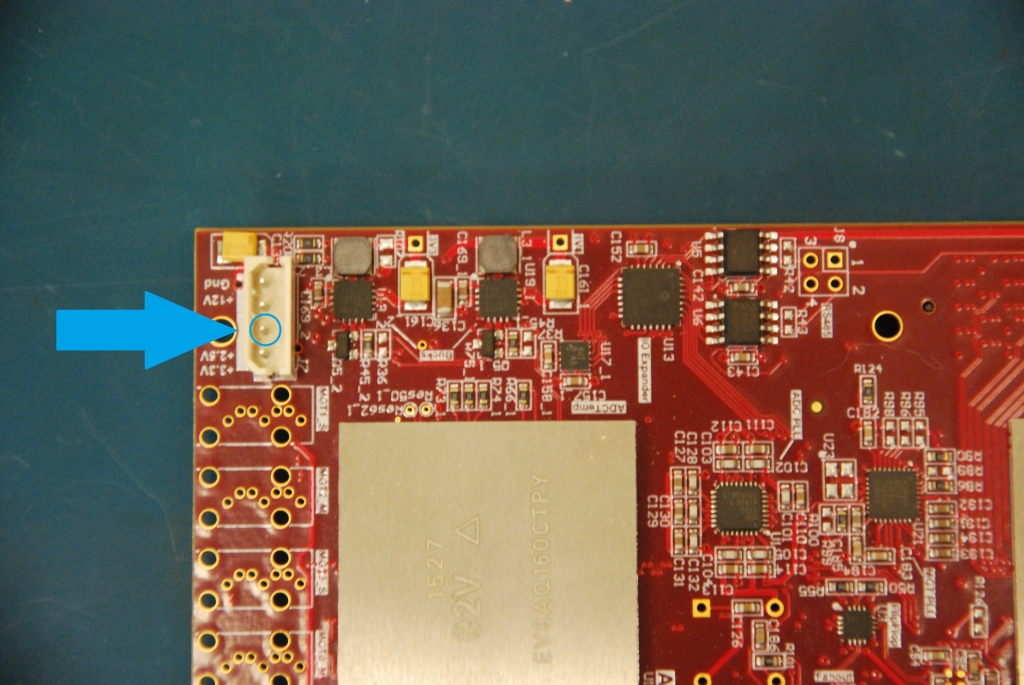
\includegraphics[width=\columnwidth]{./MezzaninePhotos/ImpedanceTest/Impedance_2V5.jpeg}
			\caption{2.5V Probe Spot - J7 Pin3}
			\label{fig:2V5Probe}
		\end{subfigure}
		\\
		
		\begin{subfigure}{0.5\textwidth}
			\centering
			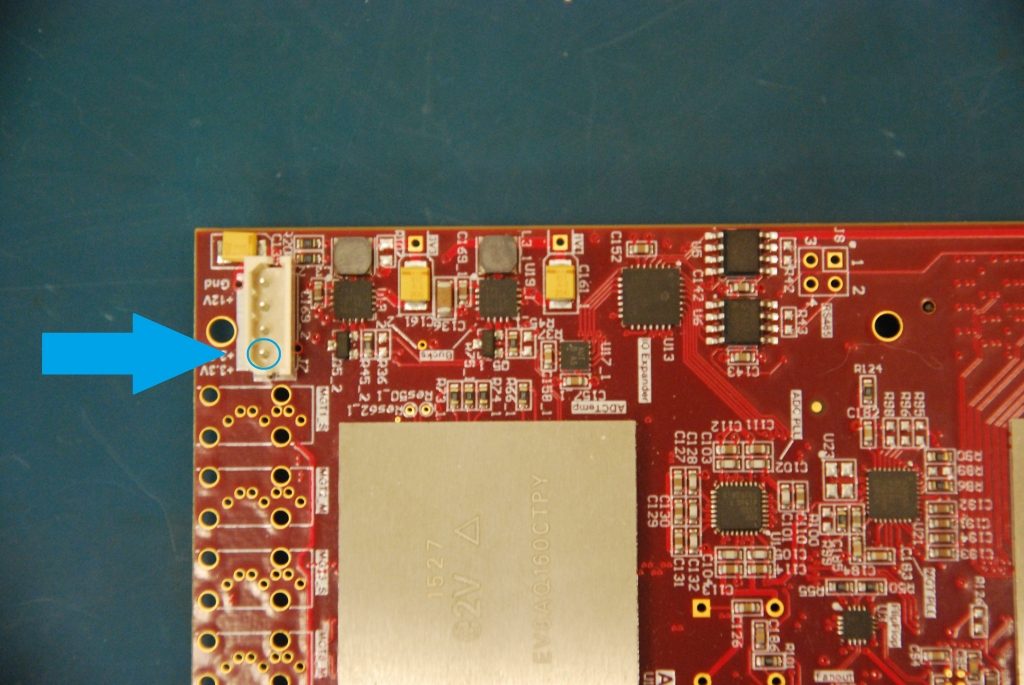
\includegraphics[width=\columnwidth]{./MezzaninePhotos/ImpedanceTest/Impedance_3V3.jpeg}
			\caption{3.3V Probe Spot - J7 Pin4}
			\label{fig:3V3Probe}
		\end{subfigure}
		&		
		\begin{subfigure}{0.5\textwidth}
			\centering
			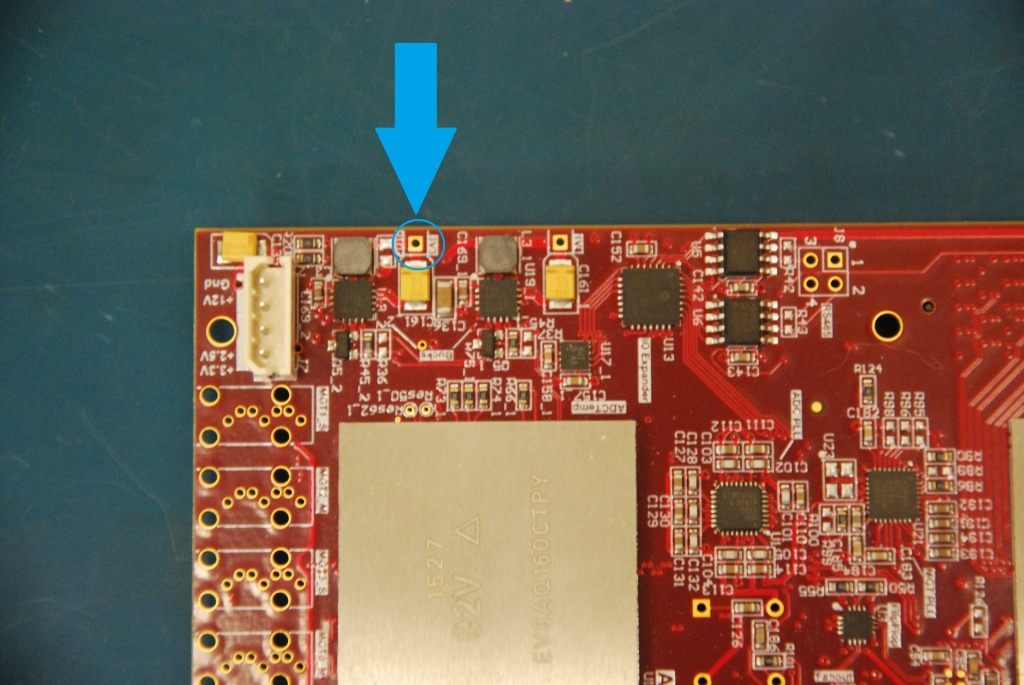
\includegraphics[width=\columnwidth]{./MezzaninePhotos/ImpedanceTest/Buck_3V3.jpeg}
			\caption{3.3V Buck Test Point}
			\label{fig:3V3BuckProbe}
		\end{subfigure}
		\\
		
		\begin{subfigure}{0.5\textwidth}
			\centering
			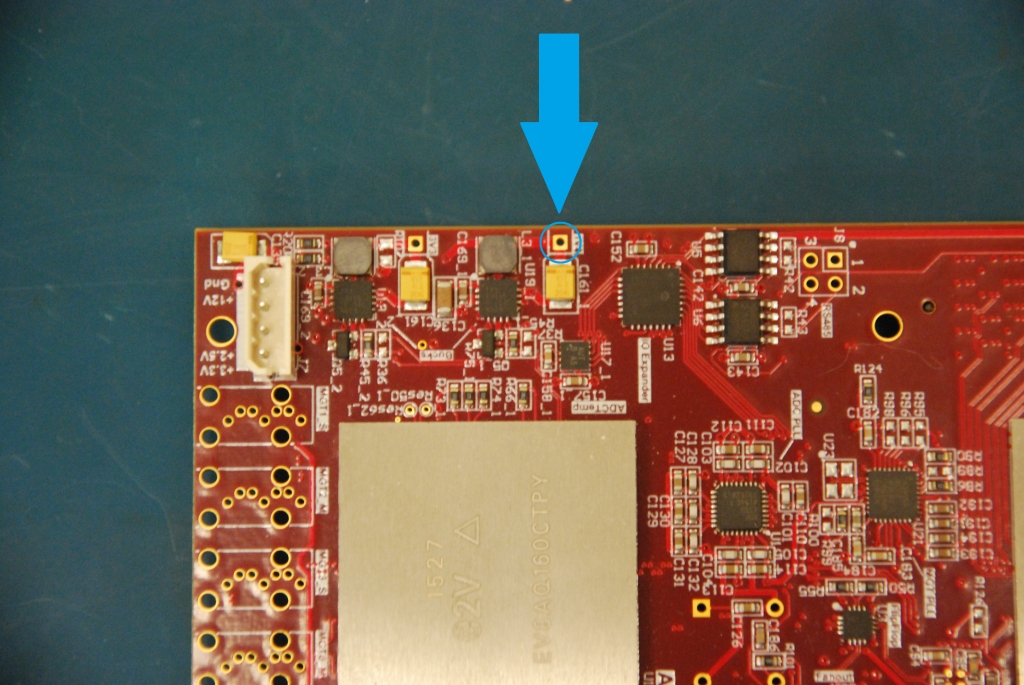
\includegraphics[width=\columnwidth]{./MezzaninePhotos/ImpedanceTest/Buck_1V8.jpeg}
			\caption{1.8V Buck Test Point}
			\label{fig:1V8BuckProbe}
		\end{subfigure}
		
	\end{tabular}
	\caption{Test points for impedance measurement}
	\label{tab:SmokeTestPoints}
\end{table}

\newpage
\subsection{Smoke Test}

Connect the SMA quick connect cable to one of the SMA ports on the mezzanine to provide ground - see figure \ref{fig:SmokeGroundLoc}.

\begin{figure}[!htbp]
	\centering
	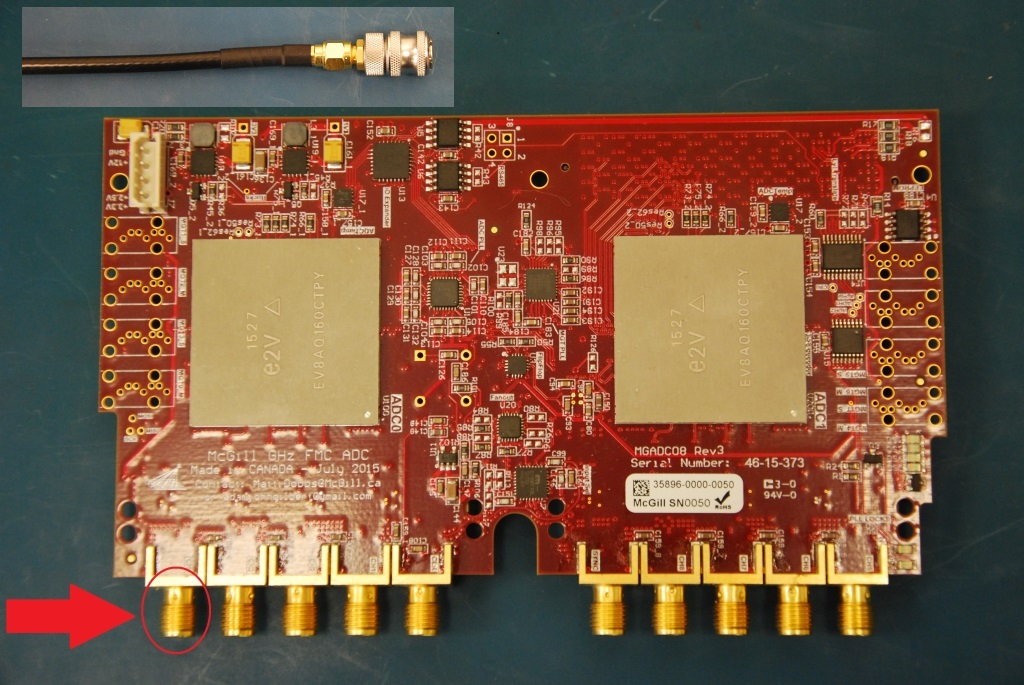
\includegraphics[height=6cm]{./MezzaninePhotos/SmokeTest/SmokeSetup.jpeg}
	\caption{Quick Connect SMA Ground Location and Quick connect SMA}
	\label{fig:SmokeGroundLoc}
\end{figure}

Connect the power cable to the mezzanine - see figure  \ref{fig:SmokeStep2}.
\begin{figure}[!htbp]
	\centering
	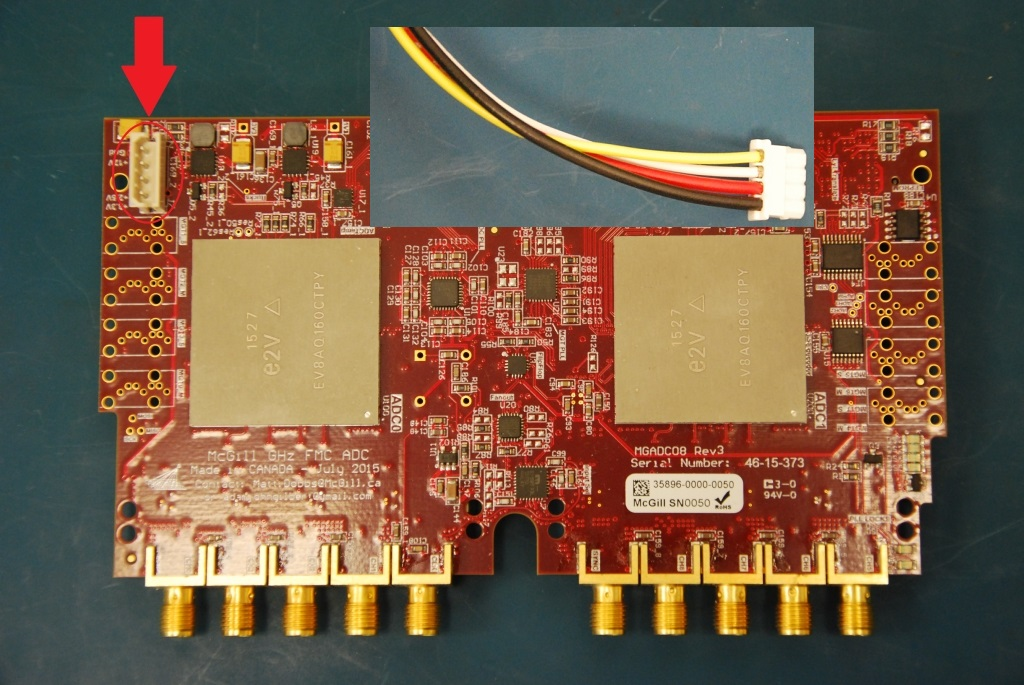
\includegraphics[height=6cm]{./MezzaninePhotos/SmokeTest/Smoke_Step1.jpeg}
	\caption{Powering the mezzanine}
	\label{fig:SmokeStep2}
\end{figure}

\newpage

\textbf{Step 1}: Check the power LED on the backside of the mezzanine - see figure  \ref{fig:SmokePowerLight}
\begin{figure}[!htbp]
	\centering
	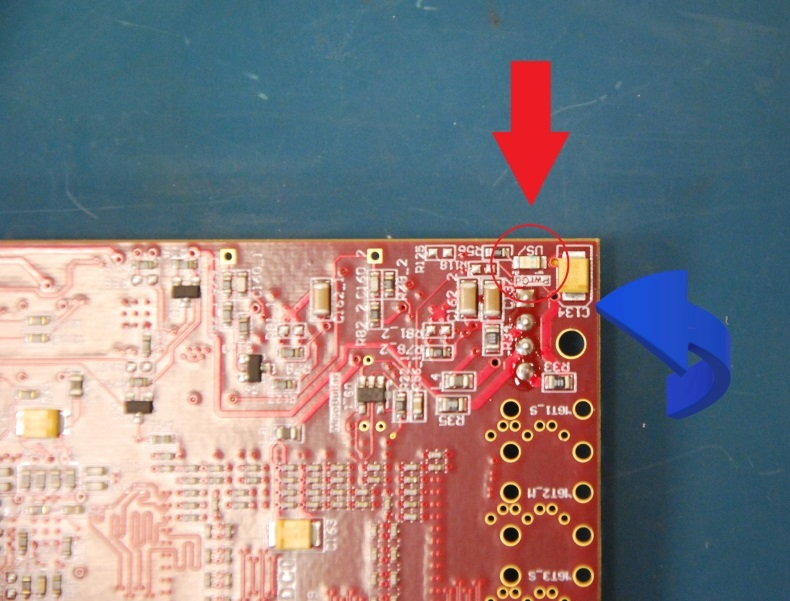
\includegraphics[height=6cm]{./MezzaninePhotos/SmokeTest/Power_Light.jpeg}
	\caption{Powering the mezzanine}
	\label{fig:SmokePowerLight}
\end{figure}

\textbf{Step 2}: Use the red probe to measure voltages as the points shown in table \ref{tab:VoltageTestPoints}
\begin{table}[!htbp]
	\begin{tabular}{cc}
		\begin{subfigure}{0.5\textwidth}
			\centering
			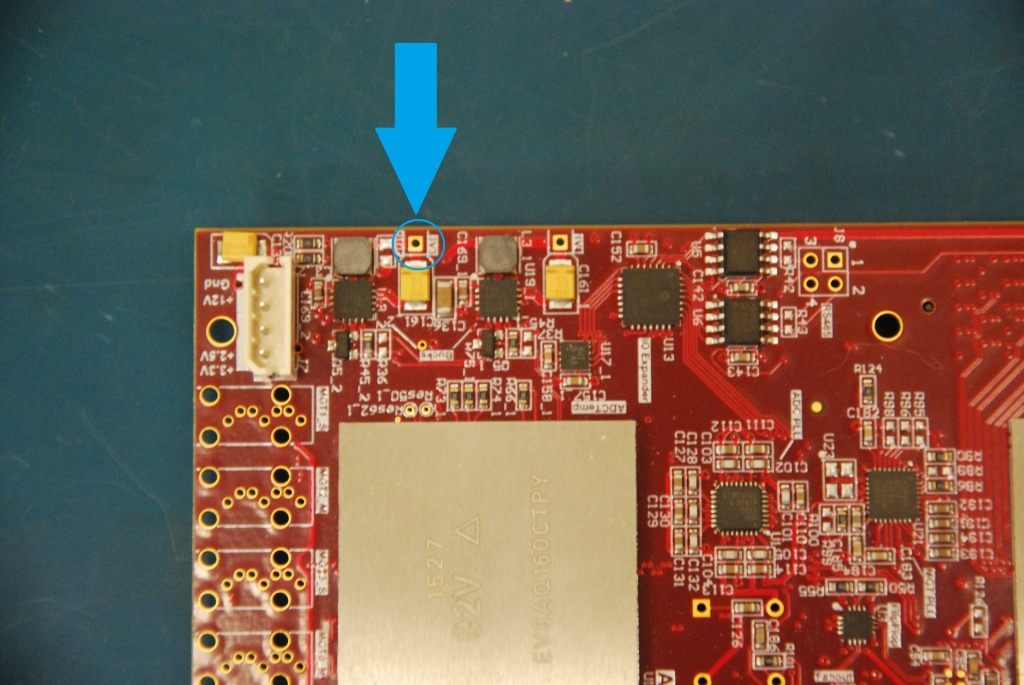
\includegraphics[width=0.9\columnwidth]{./MezzaninePhotos/SmokeTest/Smoke_3V3.jpeg}
			\caption{3.3V Buck Test Point}
			\label{fig:Smoke3V3Buck}
		\end{subfigure}
		&
		\begin{subfigure}{0.5\textwidth}
			\centering
			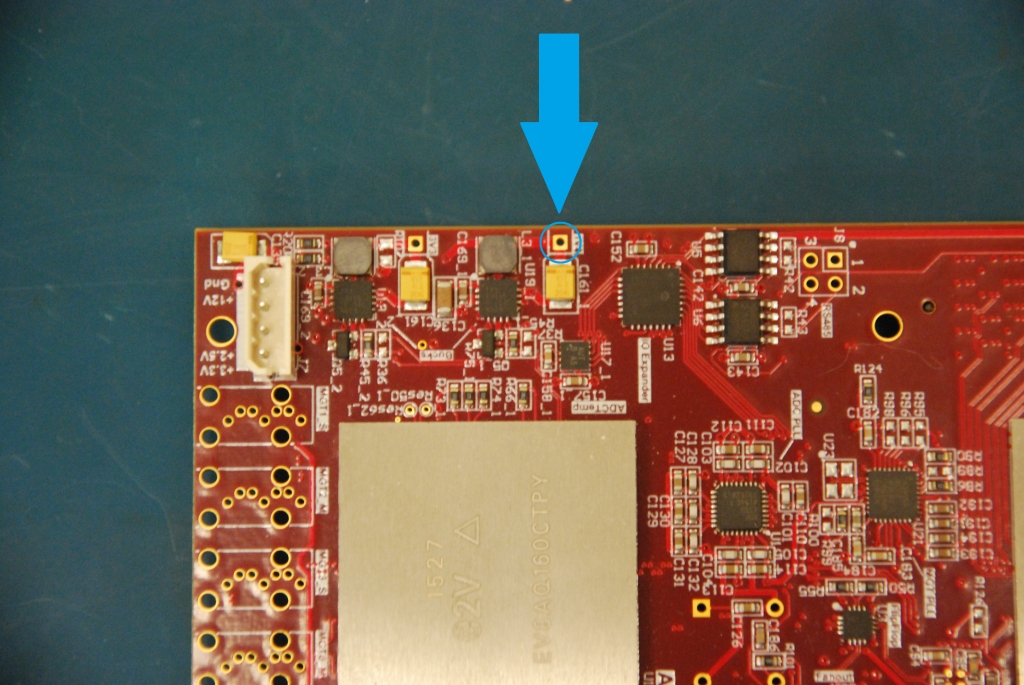
\includegraphics[width=0.9\columnwidth]{./MezzaninePhotos/SmokeTest/Smoke_1V8.jpeg}
			\caption{1.8V Buck Test Point}
			\label{fig:Smoke1V8Buck}
		\end{subfigure}
	\end{tabular}
	\caption{Test points for voltage measurement}
	\label{tab:VoltageTestPoints}
\end{table}





\pagebreak
\subsection{Carrier Tests - Mezzanine loaded onto motherboard}

For all remaining tests (EEPROM, Power, PLL , Ramp, S11), make sure that the mezzanine under test is plugged into the iceboard, and that the iceboard is able to communicate with the test computer. You will need both Ethernet cables, a valid SD card, the FPGA fan and the backplane with power cord. It's likely that we will provide you with an 'FMC Extender cable' so that the mezzanine under test is not plugged directly into the motherboard. Repeatedly changing the mezzanine may damage the motherboard connector.

\begin{figure}[!htbp]
	\centering
	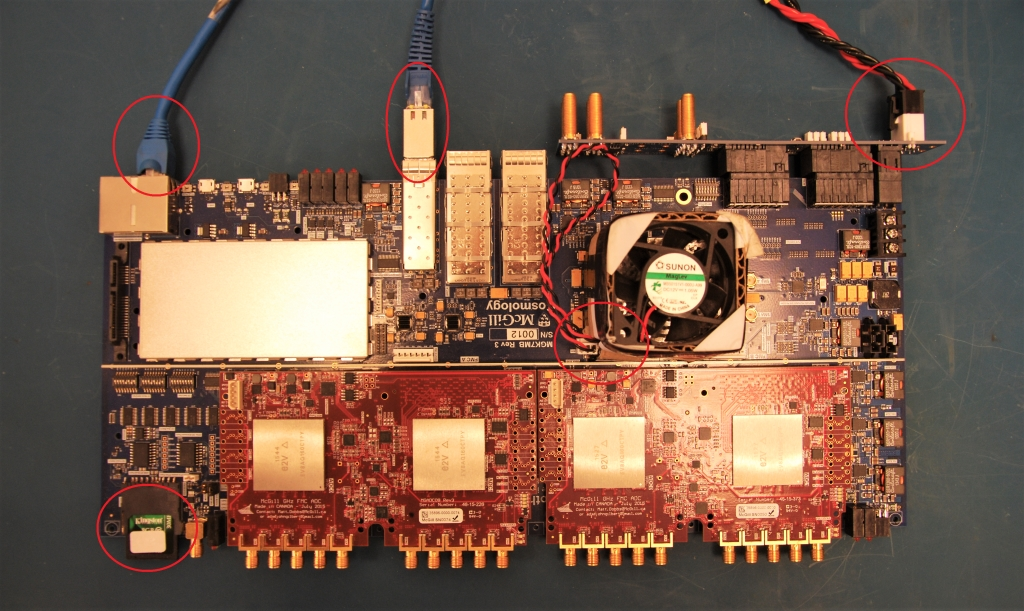
\includegraphics[height=10cm]{./MezzaninePhotos/Carrier/Carrier_tests.jpeg}
	\caption{Generic test setup when carrier board is needed}
	\label{fig:CarrierTests}
\end{figure}

\pagebreak
\subsection{EEPROM Test}
Ensure similar setup to that shown in figure \ref{fig:CarrierTests}.

\subsection{Power Test}
Ensure similar setup to that shown in figure \ref{fig:CarrierTests}.

\subsection{SPI / PLL Test}
Ensure similar setup to that shown in figure \ref{fig:CarrierTests}. Verify that the user LED's are blinking - see figure \ref{fig:SPIPLL}.

\begin{figure}[!htbp]
	\centering
	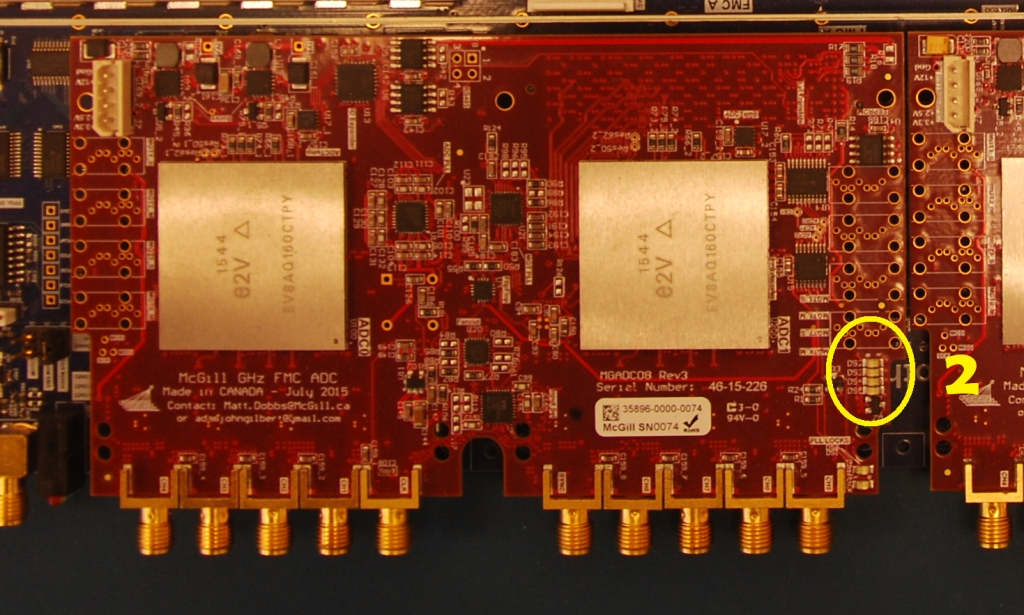
\includegraphics[width=\linewidth]{./MezzaninePhotos/PLLTest/SPI_PLL.jpeg}
	\caption{Blinking LED Locations}
	\label{fig:SPIPLL}
\end{figure}

\pagebreak
\subsection{Ramp Test}
Ensure similar setup to that shown in figure \ref{fig:CarrierTests}.

\subsection{S11}
Progressively connect the SMA quick-connect cable to the front SMA ports of the mezzanine, going through channels 1-8 in order. Note that on the mezzanine the channel ordering is 4,3,2,1 followed by 8,7,6,5 - see figure \ref{fig:S11}.

\begin{figure}[!htbp]
	\centering
	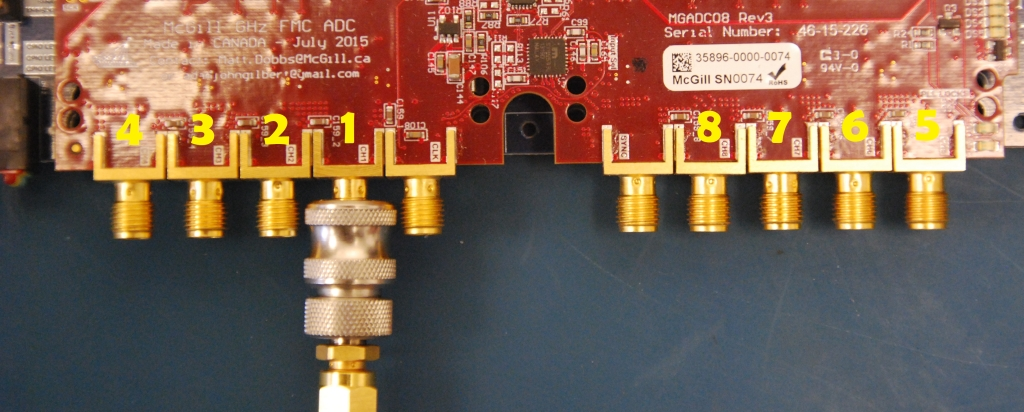
\includegraphics[width=\linewidth]{./MezzaninePhotos/S11Test/S11.jpeg}
	\caption{Channel ordering}
	\label{fig:S11}
\end{figure}


